\documentclass[../main.tex]{subfiles}
\graphicspath{{\subfix{../Images}}}

\begin{document}
\section{Introduction}
\label{sec:introduction}

For the last 15 years, blockchain has a disruptive field in academic research. The first blockchain applications available to the wider public were cryptocurrencies. These are fully digitalized currencies that can be used to abstract products and services. Cryptocurrencies use blockchain protocols to solve the double spending problem by ensuring no token can be spent more than once, therefore operating just like normal fiat currencies. In parallel with cryptocurrency projects, researchers and enthusiasts begun to experiment with a similar but functionally different token-based concept. Shortly after the release of Bitcoin, the first blockchain cryptocurrency in history, the first Non-Fungible Token project actually was based in the Namecoin blockchain, a fork from the Bitcoin project that extended the blockchain to be able to store data in its transactional database. TThe first NFT was born with the Quantum project \cite{Exmundo2023} started by digital artists Jennifer and Kevin McKoy. After creating the image depicted in Fig. \ref{fig:quantum_nft}, they wanted to sell this artwork in its digital form. The problem was to find a verifiable way to establish the provenance of the digital art. After collaborating with technology experts, they decided to register the work in the Namecoin blockchain, but using a different approach than the one used in cryptocurrencies, which was by far the main application of the early public blockchains of the 2010s. The ownership relations established by registering the image in the blockchain and "locking" its owner to a single account address at all times proved to be a critical step. In some aspects, they simply adapted the ownership mechanics of cryptocurrencies, also known as Fungible Tokens, to another type of token that could be used to represent an unique physical or digital object. The objects being represented are often unique, therefore non-fungible, hence why these tokens were named as \textit{Non-Fungible Tokens}.
\par

\begin{figure}[htp]
    \centering
    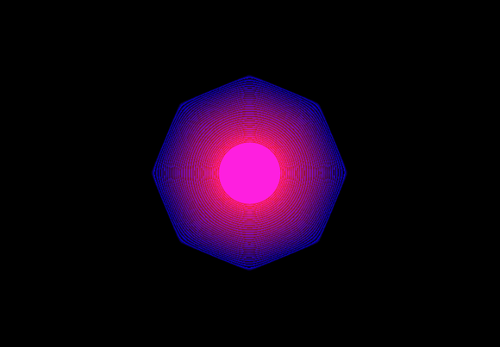
\includegraphics[width=0.9\textwidth]{../Images/02_QuantumNFT.png}
    \caption{Quantum, the first work of art to be encoded into the metadata of an NFT \cite{Exmundo2023}}
    \label{fig:quantum_nft}
\end{figure}
% // TODO: Should this image be set to grayscale for publishing?

Quantum was followed by other, arguably more successful, NFT projects, mostly establishing ownership of digital artworks. Popular projects such as \textit{CryptoPunks} \cite{nftnow2024} and the \textit{Bored Ape Yatch Club (BAYC)} \cite{Thomas2022}, followed a similar trend as Quantum. These projects created finite sets of artistic NFTs to be sold directly to users, or even given them away, as it happen during the early days of \textit{CryptoPunks} due to the unfamiliarity of transacting in cryptocurrencies. Bot projects are deployed in Ethereum and NFTs transacted in Ether (ETH), Ethereum's native cryptocurrency.
\par
Both projects minted "static" NFTs, where they encode an image directly in the token metadata (costly) or indirectly by saving the image in a distributed repository and save only a url in the NFT metadata instead (cheaper). The \textit{CryptoKitties} NFT project \cite{Dapper2017} followed the previous two but with a slight difference. Each \textit{CryptoKitty} was similar to a \textit{CryptoPunk} in the sense that the image encoded in the NFT was created from an internal parameter of the NFT, and not just some random image file. The characteristics of each \textit{CryptoKitty} were derived from an internal "genome", a 256-bit string from which substrings encoding the token characteristics (eye color, fur color, ear type, tail shape, etc.) were derived. But unlike \textit{CryptoPunks}, \textit{CryptoKitties} could be "bred" to generate new ones with characteristics derived semi-randomly from the parents genome. This dynamic, almost gaming, aspect of \textit{CryptoKitties} proved to be quite attractive to collectors and enthusiasts, which translated in a peak of NFT activity in Ethereum that pushed the network to and above its limits \cite{bbc2017}.
\par
But it was actually \textit{CryptoKitties}, an NFT project launched four years prior in 2017, that exposed the limitations of the Ethereum network, particularly regarding scalability. The team behind the project, initially named \textit{Axiom Zen} but later renamed to \textit{Dapper Labs}, tried to address these problems from withing the Ethereum framework, but with little success. It soon became clear that a new blockchain architecture was needed to fully solve these issues. Dapper Labs launch \textit{Flow} in 2020, a scalable blockchain designed from scratch with NFT applications in mind.
\par
% // TODO: Consider sending the paragraph bellow to Section 3
The approach taken with Flow is different from Ethereum from an internal perspective, but for a regular user, interacting with a Flow smart contract or NFT is not different than with any other solution. As Ethereum introduced \textit{Solidity} as the smart contract programming language for smart contracts, Flow developed \textit{Cadence} with the same purpose, albeit with a significant change in how programming principles are approached. The most glaring difference between these blockchains is how they approach data storage and ownership within the chain. Ethereum stores NFT metadata in a semi-centralised, contract-based fashion, it the sense that the smart contract address is used as a central reference point for memory referencing, and all data is stored relative to this single position. Flow has a radical approach in this sense, extending the concept of an account from just an address, as in Ethereum, to use it as a preamble to access a storage area that is unique and individual to each account. Only the owner of the account has access to digital objects stored in the associated storage area. Flow also uses a similar strategy to \textit{gas} to protect and limit the storage space associated to each account, in which the storage space available is proportional to the amount of cryptocurrency staked in that account. Just as Ethereum uses Ether (ETH), \textit{Flow} uses the \textit{FLOW} token as its cryptocurrency used to pay gas fees and to sustain the account's storage area.
\par
The fundamental architectural differences between these blockchains imply implementations that promise equal functionality but from different approaches. Also, Flow was created with the specific intention of providing an optimal solution for NFT-based projects for the current blockchain ecosystem. NFT potential is still unexplored, therefore there is value in determine which architecture provides a better alternative for a project based in these tokens. This article explores the details of both approaches and compares two similar implementations of simple NFT minting contracts towards concluding if Flow does provide a valid alternative to a more established, general purpose blockchain such as Ethereum.
\par
The rest of this article is structured as follows: Section \ref{sec:related_works} provides an overview of publications relevant to our work. In Section \ref{sec:background} we provide an introduction to concepts key to fully understand the concepts used in this publication. Section \ref{sec:solidity_ethereum_nft_implementation} details the construction and deployment of a standardised NFT Solidity smart contract in the Ethereum network, while Section \ref{sec:cadence_flow_nft_implementation} repeats the process but for the Flow blockchain and using Cadence to write the NFT contract. Section \ref{sec:results_and_comparison} provides a comparison between the two implementations, as well as the blockchains as a whole. This article concludes with Section \ref{sec:conclusion}.
\end{document}

% // TODO: Elaborate on how NFTs can be used to represent ownership of physical, real objects, not just digital ones.

% // TODO: Dynamic NFTs, or NFT 2.0, according to Barbara and Andrea's article, are very important for the downstream application but are not considered in this particular case. Check if it is a good idea to mention this at this point or later on.

% // TODO: Move a lot of the stuff here to the Background.
% // TODO: The Introduction should be short
% // TODO: The contributions of this paper must happen at the end, after the comparison